
\mychapter{Introduction}

\thispagestyle{empty}
\frenchspacing

\section{Śivadharma corpus}
\fancyhead[CE]{{\footnotesize \textit{Vṛṣasārasaṃgraha}}}
\fancyhead[CO]{{\footnotesize \textit{Introduction}}}
\fancyhead[LE]{}
\fancyhead[RE]{}
\fancyhead[LO]{}
\fancyhead[RO]{}

The \Vss\ (\VSS), a 24-chapter long Sanskrit Śaiva text,
has always%
		\footnote{For cases that seem exceptions 
		(\msKoa\ and \msPaperA\ \CHECK\ if more)
						see the manusctipt desctiptions 
						on pp.~\pageref{mss_descr}ff.}
			%	As already remarked in \mycitep{KissVolume2021}{185, n.~9}, MS G 4076 at the Asiatic Society, Calcutta, while seemingly an independent MS}
been transmitted as part of the so-called Śivadharma corpus,
in multiple-text manuscripts that usually contain 
eight texts. Much has been written recently
on the corpus itself and on the individual
texts included. 
For an introduction, an overview of secondary 
literature, an up-to-date bibliography, and the results of 
recent Śivadharma-related research, see
\mycite{SivadharmamrtaVolume2021}. 
Since the \VSS's links to other texts of the corpus, 
with the possible exception of the \DharmP, 
are relatively weak, I will refer to other
Śivadharma texts only when they are relevant
for the present inquiry.%
		\footnote{Mainly in section `\CHECK' on 
		p.~\pageref{vss_connection_other_sd_texts}}



%\section{Reading the \Vsssc}

\section{Title}\label{title}
The title \Vss%
	\footnote{Read \Vss\ for \titleface{Vṛttasārasaṅgraha}
	in \mycitep{PetechHistory}{84}.}
can be translated as:
`A Compendium on the Essence of the Bull [of Dharma].'
The last two elements (\skt{sāra-saṃgraha}) need
little explanation: this work is a 
`compendium' on, a `collection' or `summary' of (\skt{saṃgraha})
the `essence' (\skt{sāra}), of its topic. The words 
`compendium' and `collection' reflect the composite nature of
the \Vss\ well; see sections on the structure of the text and
on its possible sources on 
pp.~\pageref{structure} and 
pp.~\pageref{vss_connection_other_texts}ff. 
The\label{bull} remaining question is whether the bull in the title 
is only a reference to a representation of Dharma 
or also a hint at Śiva's bull, his vehicle or mount, 
sometimes called Nandi or Nandin in other works.%
		\footnote{There is no trace of Nandi/Nandin
		as identified with the bull in the \Vss.
		On the possible time after which 
		Nandi or Nandin, originally a \cskt{gaṇa}{gana} 
		was considered a \csindex{bull}, see 
		\mycite{bhattacharya_nandin_1977} and 
		\mycitep{Pancavaranastava}{100--108 and 171--172}.}

Dharma is frequently referred to as a (four-legged) 
bull, often as one that loses a leg in every Kalpa,
in Dharma literature from at least the time of the \MBh,
see, e.g., \MBH\ 3.188.10--12; and \Manu\ 1.81a 
(\skt{catuṣpāt sakalo dharmaḥ} and 8.16a: 
\skt{vṛṣo hi bhagavān dharma}.% 
	 \footnote{See, e.g., \mycite{CoutureDharma}; also  
	 \mycite{GutierrezEmbodiment} 
	 (in the section `In animal terms'): 
	 `The emphasis on the whole body, with all four legs, assures 
	 the maintenance of stability in dharma's structure, which in 
	 turn structured Brahmanical society.'}

In addition, in Śaiva contexts, the bull of Dharma
does feature as Śiva's vehicle. See, e.g., 
\mycitep{BakkerWorld2014}{68ff}, especially p.~69,
where Bakker, after analysing seals containing images of
bulls, remarks:


\begin{quote}
The topicality of the Śaiva accommodation 
of the Dharma in the second half of the 
sixth century is nicely illustrated by a myth found in the
original \titleface{Skandapurāṇa} [\dots]
the uncontrollable, wild bull \ie{vṛṣa} is 
domesticated by Śiva's Gaṇapa Prabhākara [\dots]
In this way the bull is transformed into Śiva’s vehicle \ie{vāhana}. 
\end{quote}

\noindent
Or putting it more bluntly: 

\begin{quote}
Making the bull Śiva's vehicle implies that Śiva has become
the supreme lord of the Dharma, or that the Dharma has 
been accommodated in [Ś]aivism.%
	\footnote{\mycitep{SkandaIIb}{65 n.~210}.
	\citeauthor{bhattacharya_nandin_1977} 		
			(\citeyear{bhattacharya_nandin_1977}, {1552}) 
			suggests that `In the Purāṇas the bull
		(\csindexxx{Vṛṣabha}{vrsabha}{\skt{vṛṣabha}} or 
		\csindexxx{Vṛṣa}{vrsa}{\skt{vṛṣa}}) 
	of Śiva is identified with Dharma, ``virtue personified''. 
		This is a new development to sanctify the animal 
		vehicle of the god. This new situation took place with the 		
		religious rite when an offering of a bull to a Brahmin   
		deemed to be	of a high religious merit.'}
\end{quote}

\noindent
The possibility that the bull in the title \Vss\ refers 
not only to Dharma as a bull, but also
to Śiva's \skt{vāhana} has been mentioned
in \mycitep{UmaSivaPlay}{238 n.~13}, and briefly
discussed in \mycitep{KissVolume2021}{185--186} 
with the conclusion that although 

\begin{quote} 
while the bull as a synonym of Dharma is mentioned in 
the text repeatedly, [\dots]
there is no clear reference to Śiva's mount in the [\VSS, it is] 
not inconceivable that the redactors of the \Vss\ had 
the same association in mind, namely that the bull in 
question is both Dharma and Śi­va's mount.%
	\footnote{Note that \SDhU\  12.87
				also mentions the `Dharma bull':
	    \skt{īśvarāyatanasyādhaḥ śrīmān dharmavṛṣaḥ sthitaḥ} |
    	\skt{yatra vīravṛṣas tatra kṣityāṃ gomātaraḥ sthitā} || }
\end{quote} 

%Śiva got his bull, MBh:
%13076027a vṛṣabhaṃ ca dadau tasmai saha tābhiḥ prajāpatiḥ
%13076027c prasādayām āsa manas tena rudrasya bhārata
%13076028a prītaś cāpi mahādevaś cakāra vṛṣabhaṃ tadā
%13076028c dhvajaṃ ca vāhanaṃ caiva tasmāt sa vṛṣabhadhvajaḥ
%13076029a tato devair mahādevas tadā paśupatiḥ kṛtaḥ
%13076029c īśvaraḥ sa gavāṃ madhye vṛṣāṅka iti cocyate

%MMW `vṛṣa':\\
%``Justice or Virtue personified as a bull or as''Siva's bull Mn. viii,
%16 Pur. Kāvyād.; just or virtuous act, virtue, moral merit ``Siś.
%Vās.;''

%Mahākṣapaṇaka's koṣa (CHECK date), the Anekārthadhvanimañjarī, places
%the meaning `dharma' as first when defining the word `vṛṣa':
%
%\begin{quote}
%    \skt{dharmo vṛṣo vṛṣaḥ śreṣṭho vṛṣo gaur mūṣiko vṛṣaḥ} |\\
%    \skt{vṛṣo balaṃ vṛṣaḥ kāmo vṛṣalo vṛṣa ucyate} || 1.48
%    \end{quote}

% Śivapurāṇa:
% śuddhasphaṭikasaṃkāśo vṛṣabhaḥ sarvasundaraḥ ||
% yo dharma ucyate vedaiḥ śāstraiḥ siddhamaharṣibhiḥ ||54||
% tam ārūḍho mahādevo vṛṣabhaṃ dharmavatsalaḥ||
% śuśubhe 'tīva devarṣisevitaḥ sakalair vrajan ||55||


%visnusmrḍn:ViS 86.15a/ vṛṣo hi bhagavān dharmaś catuṣ-pādaḥ prakīrtitaḥ
%/
%
%Śivapurāṇa 2.3.40.54--55:
%
%\begin{quote}
%\skt{śuddhasphaṭikasaṃkāśo vṛṣabhaḥ sarvasundaraḥ} |\\
%\skt{yo dharma ucyate vedaiḥ śāstraiḥ siddhamaharṣibhiḥ} ||\\
%\skt{tam ārūḍho mahādevo vṛṣabhaṃ dharmavatsalaḥ} |\\
%\skt{śuśubhe 'tīva devarṣisevitaḥ sakalair vrajan} ||
%\end{quote}
%also quoted by \mycitep{bhattacharya_nandin_1977}{1553}	

%smrti/dharma/krtyaratnaakara.dn: !!! dharmo 'yaṃ vṛṣarūpeṇa nāmnā
%nandīśavaro vibhuḥ \textbar{} dharmān māheśvarān vakṣyaty ataḥ prabhṛti
%nārada\textbar{}\textbar{}
%
%tak2015/AtmapujaT55Muktabodha.dn: dharmas tatra vṛṣākāro jñānaḥ
%siṃhasvarūpakaḥ \textbar{} vairāgyaṃ

%On the title, see 
%\mycite{DeSiminiMSSFromNepal2016} (238, n.\thinspace 13):
% `'As noted by \Sanderson\
%{[}\ldots{}{]}, this title can have a double meaning, since the `bull'
%(vṛṣa) is both a synonym of `religious practice' and the traditional
%mount (vāhana) of Śiva. i.e.~Sanderson (Forthc. b), Śaivism and
%Brahmanism. (can't find it)

\noindent
\mycite{SandersonTolerance2015} (210 n.~136), 
says the following on \cskt{vṛṣa}{vrsa} being Dharma
in general, and on the bull appearing on the coins of the 
Hephthalite Hun Mihirakula in particular, also
mentioning the \VSS: 

\begin{quote}
To laud the bull (\cskt{vṛṣa}{vrsa}) 
would be surprising if the intended meaning were 
the bull that is Śiva's mount, but not if the word is intended in its figurative meaning, namely \skt{dharmaḥ}, 
or \skt{sukṛtam} `the virtuous actions [prescribed by
the Veda].' For this meaning of \skt{vṛṣaḥ} see, for example,
Amarasiṃha, \skttitle{Nāmaliṅgānuśāsana}{Namalinganusasana} 
1.4.25b (\skt{sukṛtam vṛṣaḥ}),
3.3.220 (\skt{sukṛte vṛṣabhe vṛṣaḥ}); 
Halāyudha,
\skttitle{Abhidhānaratnamālā}{Abhidhanaratnamala} 1.125cd (\skt{dharmaḥ puṇyaṃ vṛṣaḥ śreyaḥ
sukṛtaṃ ca samaṃ smṛtam}); 
\Manu\ 8[.]16a
(\skt{vṛṣo hi bhagavān dharmas}\dots); 
and the Gwalior Museum Stone
Inscription of Pataṅgaśambhu (\mycite{MirashiGwalior1962}), l. 15,
\skt{vṛṣaikaniṣṭho `pi jitasmaro 'pi yaḥ śaṅkaro 'bhūd 
bhuvi ko 'py apūrvvaḥ}, 
concerning the Śaiva ascetic Vyomaśambhu: 
`He was in the
world an extraordinary new Śiva, since he too was 
\skt{vṛṣaikaniṣṭhaḥ}
(`devoted solely to pious observance'; 
in Śiva's case `riding only on the Bull') and he too was 
\skt{jitasmaraḥ} (`one who had defeated sensual
urges'; in Śiva's case `the defeater of the Love god Kāmadeva'). 
This is also the meaning of \skt{vṛṣaḥ} in the title \Vss,
one of the works of the Śivadharma corpus 
(see, e.g., \mycitep{SandersonSaivaLit2014}{p.~2}), i.e., 
`Summary of the Essentials of the [Śiva]dharma'. 
\end{quote}

\noindent
In the last sentence here, \Sanderson\ implies that the
\Vss\ is organically part of the teachings that we 
may collectively call the Śivadharma, and he
thus supplies `Śiva' when translating the title 
\Vss. A closer examination of the \VSS\ 
reveals no direct references to either Śiva's bull or
to the bull as embodying the Śivadharma. Instead, the bull
in the \VSS\ is repeatedly associated with the Dharma that
is the four \asrama s (see p. \pageref{bullasfourasramas}).
My conclusion is that while the word \cskt{vṛṣa}{vrsa} in the
title may well carry a reference to Śiva's bull, it is always
only implied and never explicitely taught, while the bull as
the personification of Dharma as the four
\asrama s explicitely appears. Thus
the title actually lacks any explicit hint to Śaivism,%
	\footnote{In contrast with, e.g., the \UUMS\ 
					\msCa\ fol.~184r ll. 3--4 (see
					\mycitep{KissVolume2021}{185--186}):
		\skt{īśvara uvāca |
  			na jānanti ca loke 'smin mānavā mūḍhacetasaḥ |
 			catuṣpādo bhaved dharmaḥ śuklo 'yaṃ mama vāhanaḥ 
 									||}}
 which
fits in well with the rather blurred and multi-layered 
affiliation of the text to Dharmaśāstra, Vaiṣṇavism and Śaivism.%
		 \footnote{See p.~\pageref{structure}.}
%		\footnote{See also \mycitep{BakkerWorld2014}{69}, who 
%			while discussing a seal of Śarvavarman that 
%			features a beautifully carved bull representing Dharma,
%			remarks (italics mine): `The reader \textit{may} also see in the 
%			image the thriving Śaiva religion, represented
%			by the Bull, the vāhana of Śiva [\dots]'} 




%\mysubsubsection{Vṛṣadeva's commission?}{vrsadevas-commission}
Finally, as a fanciful experiment, and if one accepts 
that the \VSS\ originated in Nepal,%
		\footnote{See  \CHECK} 
one could wonder if the title \Vss\ 
has anything to do with the Licchavī king Vṛṣadeva.
\citeauthor{SandersonSaivaAge} 
(\citeyear{SandersonSaivaAge}, 74) mentions that  
Vṛṣadeva is `described in an inscription of his eighth-century 
descendant Jayadeva as having inclined towards Buddhism;%
			 \footnote{See \mycitep{Vajracarya1973}{148, l. 9}: 
					\skt{sugataśāsanapakṣapātī}.}
a view confirmed by a local chronicle, which attributes to
him the establishing of Buddhist images,'
%fn: Lévi 1990, vol. 2, p. 98.
and that this king established 
`the Caitya of the Sı̄nagu-vihāra (the Svayambhūnāth Caitya).'
More importantly, Sanderson summarises the 
information to be found in the 
Changu Narayana Pillar Inscription (east shaft),%
		\footnote{\mycitep{GnoliNepInscr}{1},  and 
		https://siddham.network/inscription/in02001/} 
namely that Vṛṣadeva was the great-grandfather of Mānadeva, whose
`dated inscriptions range in date from 459 to 505/6' [\CE]
(\mycitep{SandersonSaivaAge}{75}).
%	   \footnote{Vṛṣadeva was succeeded by Śaṅkaradeva and   		            Dharmadeva.}
This would place 
the reign of Vṛṣadeva around 400 \CE. 
The early fifth century may look too early for the date of composition
of the \Vss, and any connection between this king
and the text is impossible to prove at the moment, 
but it is equally impossible to reject it fully, 
and if there were any connection, 
it would serve as explanation for the slightly
unusual nature of the title (`\dots\ the essence of the bull').
\hide{
%https://siddham.network/inscription/in02087/
%https://siddham.network/inscription/in02087/?section=translation
%https://siddham.network/inscription/in02002/
%https://siddham.network/inscription/in02001/
%https://infogalactic.com/info/Licchavi_(kingdom):
}

%
%Gopālarājavaṃśāvalī p. 124 Dharmadeva and a vṛṣa statue? Text mentions vṛṣadhvaja though...
%
%Pañcāvaraṇastava 71:
%pratyag āśāsthitaṃ vande vṛṣaṃ ca vṛṣabhākṛtim|
%sākṣād dharmaṃ sitaṃ tryakṣaṃ parameśasya vāhanam||
%+ notes to this verse on p. 171
\section{Genre}

Is the \VSS\ a Purāṇa? There are at least two reasons to think so.
One is the section \VSS\ 1.62--75, a list of so-called \skt{vedavyāsa}s, 
transmitters of Purāṇas, from Brahmā, to Vyāsa Dvaipāyana, Romaharṣa and 
his son. Why should a text include in its first chapter such a list other than to imply that it describes its own origins?

Another argument is that the topics dealt with in the \VSS\ are exactly what
we expect from a Purāṇa. The famous \skt{purāṇapañcalakṣaṇa} includes,
following Wilson's translation (in \mycitep{RocherPuranas1986}{26}), the following:
(1) primary creation, cosmogony and chronology (\skt{sarga}); 
(2) creation, destruction of the world (\skt{pratisarga});
(3) geneologies (\skt{vaṃśa}); 
(4) Manu eras (\skt{manvantara}s);
(5) history (\skt{vaṃśānucarita}).%
		\footnote{See, e.g., \SIVP\ 7.1.41: 
				\skt{sargaś ca pratisargaś ca 
						vaṃśo manvantarāṇi ca |
                        vaṃśānucaritaṃ caiva 
                        purāṇaṃ paṃcalakṣaṇam} ||}
Arguably all these are present in the \VSS, most of them already in chapter one, and later in twenty-one and
twenty-four, plus narratives of the deeds of gods (e.g. in chapter twenty-three), and much more. It is possible
that some parts of the \VSS\ were originally intended
to form a \skt{purāṇa}. The part in question could
the the outermost layer of the text. This leads us
to the examination of the structure of the \VSS.

%Hazra. \verify\ Brahmāṇḍapurāṇa is similar \verify

Alternatively, is the \VSS\ a Dharmaśāstra?  It does have features  
that are characteristic of Dharmaśāstric texts such as
descriptions of rules of conduct (chapters 3--8), discussions
of the \skt{varṇa}s and \skt{āśrama}s (chapters 11 and 19),
but some important elements such as narratives (chapter 12),
yogic teachings (chapter 16), lists of \skt{tīrtha}s (chapter 10),
and the frequent use of poetic metres (e.g. \skt{upajāti} and
\skt{śārdūlavikrīḍita}) seem alien to Dharmaśāstra.

\Fol251v of \msPaperA\ contains a scribal addition that 
gives a richer and somewhat more nuanced definition of the genre of the \VSS, 
paraphrasing \MBh\ 1.56.21:%
			\footnote{\MBh\ 1.56.21 reads:
									\skt{arthaśāstram idaṃ puṇyaṃ dharmaśāstram idaṃ param |
		                              mokṣaśāstram idaṃ proktaṃ vyāsenāmitabuddhinā ||}. 
		                              The parallel between the scribal verses in \msPaperA\ and the 
		                              \MBh\ has already been noted in 
		                              \mycitep{DeSiminiMSSFromNepal2016}{253 n.~51}.}

\begin{quote}
\skt{pādam ādyam}% 
		\footnote{Understand \skt{pādamātram}?}
							\skt{idaṃ śāstraṃ yo 'dhīyīta jitendriyaḥ |}\\
\skt{tenādhītaṃ sarvvadharmmam iti nāsty atra saṃśayaḥ ||}\\
\skt{arthaśāstram idaṃ puṇyaṃ dharmmaśāstram idaṃ paraṃ |}\\
\skt{mokṣaśāstram idaṃ proktaṃ śivenāmitatejasā |}

Should someone read [only as much as] the first \skt{pāda} [of]
this \skt{śāstra} with his senses subdued, [that would count as if]
he read all the Dharmi[c teachings], no doubt about this.
This virtuous Arthaśāstra, this excellent Dharmaśāstra, 
this \skt{śāstra} on Liberation was taught by Śiva, whose splendour is
unmeasurable.
\end{quote}

\noindent
According to this definition, the \VSS\ is both an Arthaśāstra and a
Dharmaśāstra, and also a yogic text that gives instructions on \skt{mokṣa}.




\section{Structure}\label{structure}

As described in \mycitep{KissVolume2021} in
more detail at least three structural 
layers can be discerned in the \VSS:
a general, Dharmaśāstric one; a more or less Vaiṣṇava one; 
and a Śaiva one. Figure \ref{fig:struct2021} is
a diagramme reproduced from 
\mycitep{KissVolume2021}{188}
showing the textual divisions more precisely.

\begin{figure}
\begin{tikzpicture}
\path  (0,0) coordinate(A);
\draw [scale=1,shift={(0,0)}] (-.9,.6) arc [start angle=160, end angle=20, radius=2];
\draw [scale=1,shift={(0,0)}] (-.2,.5) arc [start angle=160, end angle=20, radius=1.3];
\draw [scale=1,shift={(0,0)}] (-.2,-.5) arc [start angle=200, end angle=340, radius=1.3];
\draw [scale=1,shift={(0,0)}] (-.9,-.6) arc [start angle=200, end angle=340, radius=2];
% circles
%\draw [scale=1,shift={(0,0)}] (1,0) circle (2);
%\draw [scale=1,shift={(0,0)}] (1,0) circle (1.3);
\draw [scale=1,shift={(0,0)}] (1,0) circle (.6);
\draw[decoration={text along path, text={General Dharma{ś}{ā}stric},raise=.8,text align=center}, decorate] (-0.5,0) arc [start angle=180,end angle=0,radius=1.5];
\draw[decoration={text along path, text={General Dharma{ś}{ā}stric},raise=.8,text align=center}, decorate] (2.5,0) arc [start angle=360,end angle=181,radius=1.5];
\draw[decoration={text along path, text={Vai{ṣ}{ṇ}ava},raise=.8,text align=center}, decorate] (0,-.2) arc [start angle=180,end angle=0,radius=1];
\draw[decoration={text along path, text={Vai{ṣ}{ṇ}ava},raise=-.5,text align=center}, decorate] (2,.1) arc [start angle=360,end angle=180,radius=1];
\node at (1,0) {{Ś}aiva};

        % arrows
        \draw [->, line width=0.25mm] (2,1.5) -- (5,1.5);
        \draw [->, line width=0.25mm] (1.9,.4) -- (5,0.4);
        \draw [->, line width=0.25mm] (1.2,-0.3) -- (5,-0.3);
        \draw [->, line width=0.25mm] (1.55,-1) -- (5,-1);
        \draw [->, line width=0.25mm] (1.25,-1.8) -- (5,-1.8);

\node[text width=5cm] at (8,1.5)  {verses 1.1--8};
\node[text width=5cm] at (8,0.4)  {verses 1.9--10.3};
\node[text width=5cm] at (8,-0.3) {verses 10.4--18.46};
\node[text width=5cm] at (8,-1)   {verses 19.1--21.29};
\node[text width=5cm] at (8,-1.8) {verses 21.30--24.83};

%vertical lines
        %\draw [line width=0.5mm] (-1,0) -- (0.4,0); 
        %\draw [line width=0.5mm] (1.6,0) -- (3,0); 

% \path  (0,0) coordinate(A); \draw [scale=1,shift={(0,0)}] (6,0) circle (2); \draw [scale=1,shift={(0,0)}] (6,0) circle (1.3); \draw [scale=1,shift={(0,0)}] (6,0) circle (.6); \draw[decoration={text along path, text={As a legendary yogin},raise=.8,text align=center}, decorate] (4.5,0) arc [start angle=180,end angle=0,radius=1.5]; \draw[decoration={text along path, text={As an interlocutor},raise=.8,text align=center}, decorate] (5,-.2) arc [start angle=180,end angle=0,radius=1]; \node at (6,0) {As sacrifice};

\end{tikzpicture}
\caption[Structure of the \VSS]{The structure of the \VSS\ (reproduced from \mycitep{KissVolume2021}{188})\label{fig:struct2021}}
\end{figure}

Each layer is characterised by a dialogue between
two interlocutors. The layer that I label general 
Dharmaśāstric is a dialogue between Janamejaya and
Vaiśampāyana; the Vaiṣṇava layer is presented as
a dialogue between Vigatarāga, who is
Viṣṇu in disguise, and Anarthayajña,\label{anarthayajna_person} the ascetic;
the Śaiva layer is a dialogue between Śiva and Devī,
as related by Nandikeśvara.

Another way to represent the overall structure of the \VSS\
visually is shown by Figure \ref{fig:structlotus} 
on p.~\pageref{fig:structlotus} below. 
The \VSS\ is represented
as a lotus whose petals represent chapters. White petals indicate chapters within
the general Dharmaśāstric layer; light grey colour
indicates the Vaiṣṇava layer; dark grey colour indicates
Śaiva chapters. The divisions are not clear-cut: 
the first few verses of chapter one belong to
the general layer and there are some transitions
within chapters. Also, the layers are not hermetically
sealed, and there is some `leaking' between the chapters.
Śaiva chapters do contain Vaiṣṇava material and vice versa.
The labels next to the petals are keywords that indicate
the main topic of the individual chapters. Big check marks
indicate the presence of Anarthayajña the ascetic in
the given chapter, while smaller check marks indicate
references in the given chapters to Anarthayajña's
ascetic practice repeatedly called \skt{anartha-yajña}, 
i.e.\ `non-material\thinspace /\thinspace internali\-sed sacrifice/worship.'
Anarthayajña in both senses seems to be one of the 
main foci of the \VSS. A brief overview of 
the Vaiṣṇava chapters would be the following.
Anarthayajña, a Vaiṣṇava ascetic, who propagates 
a system of internalised \skt{āśrama}s\thinspace /\thinspace
a system beyond the traditional \skt{āśrama}s, 
and who was born into an obscure or fluid \skt{varṇa} 
(\skt{brāhmaṇa\thinspace /\thinspace kṣatriya}),
who is also a propagator of a Śaiva(?) version of 
internalised sacrifice or worship, is
being tested by Viṣṇu; he passes the test
and follows Viṣṇu to Viṣṇuloka.

Another general observation
could be that around one fourth of the text is
an elaboration on rules of religious conduct 
\ie{yama-niyama}. Also, chapter two seems slightly
out of place, being a clearly Śaiva chapter inserted
in the Vaiṣṇava layer and in the corresponding 
dialogue of the Vai\-ṣṇa\-va interlocutors, so to say.
On these, see \mycitep{KissVolume2021}
and the analyses of the individual chapters below.





%{\Huge\textsc{The V\textsubring{r}ṣasārasaṀgraha: Structure}}\hfill Csaba Kiss, 2 Mar 2022, Dharma Workshop, Berlin
\begin{figure}[!]

\begin{center}
\thispagestyle{empty}
\vspace{0em}
\leftskip-7em
\begin{tikzpicture}[scale=1]
%\bigcircle
\drawpetalswitharrows  
\colorpetalsOne
\drawtopicsTwo
\textTwo
\end{tikzpicture}
\end{center}

\caption[Structure and topics of the \VSS]{The structure and topics of the \VSS\ 
   \label{fig:structlotus}}
   
\end{figure}



\section{Connection to other texts}
\label{vss_connection_other_texts}

The \VSS's debt to the \MBh\ (\MBH) is evident right
from its first few verses. As already noted in, 
the frame story in the \VSS\  comprises

\begin{quote}
a dialogue between Janamejaya and Vaiśampāyana, 
echoing the setting of the frame story of the \MBh. 
Janamejaya is the king at whose snake-sacrifice 
Vaiśampāyana recited the whole \MBh\ for the first
time. This important moment is where the frame story 
of the \Vss\ takes off: Janamejaya has 
listened to the whole of the \MBh,
but having had the desire to hear the ultimate 
teaching on Dharma, he is bound to remain unsatisfied.
 Asked by Janamejaya for a higher teaching
on Dharma which can lead to liberation, 
Vaiśampāyana relates a dialogue between Vigatarāga 
(in fact Viṣṇu in disguise) and Anarthayajña, an ascet­ic.%
				\footnote{\mycitep{KissVolume2021}{187}}
\end{quote}
 
\noindent
Thus the frame story in the \VSS\ suggests
that the text is to be ideally read as a summary 
or higher synthesis of the Dharmic teachings found
in the \MBH. The \VSS's connection to the \MBH\
is also evident from quotations from and paraphrases
of \MBH\ passages. EXAMPLES (tattvasystem).
  References to other works - Mahābhārata - nakule - vipule etc.

Moreover, a significant number of passages in 
the \VSS\ derive from Purāṇas and from \Manu. EXAMPLES.

The possibility of influence from Śaiva tantric works is
minimal, but not to be excluded. EXAMPLES.
Niśvāsakārikā



Śivadharma texts:
\label{vss_connection_other_sd_texts}


Embryology

yoga \DharmP\ see below
Dhyāna in the \VSS\ and the \DHARMP
\label{dharmaputrika}

Compare, borrowings

Bṛhatkālottara,








\section{Dating and provenance}
\label{provenance}
There are a number of reasons to think that
Nepal, or the Kathmandu valley, is the main
candidate for being the \VSS's place of composition
or final redaction. As for the time it may have 
happened, the first half of the period in the history of Nepal 
that is the most poorly documented and is thus 
variably labelled `the transitional period,'%
	\footnote{\mycitep{PetechHistory}{31}}
or a `relatively obscure period [\dots]
[b]etween the Licchavis, who last appear 
in epiraphical record in 737 [\CE], 
and the Malla kings, who ruled from 1200--1768',%
	\footnote{\mycitep{SandersonSaivaAge}{77}}
is the most probable one.

To make assumptions about the place of 
composition of the \VSS, we can consider 
the following: the location of the manuscript 
evidence, place names and individuals  
mentioned in the text, and a possible influence
of any local language on the style and grammar
of the text.

All MSS known to us that transmits the \VSS\ 
hail from Nepal. This in itself is not strong evidence
but it stands in stark contrast with the MSS situation
of the \SDHS\ and the \SDHU.%
		\footnote{See, e.g., \mycitep{UmaSivaPlay}{589}.}

The geographical locations 
mentioned in the \VSS\ include the
\skt{tīrtha}s mentioned in chapter ten:
Himavat (the Himālayas),
Kurukṣetra,
Prayāga,
Vārāṇasī,
Yamunā,
Gaṅgā,
Agnitīrtha, % north
Somatīrtha, % north
Sūryatīrtha, % north
Puṣkara, % north
Mānasa, % north
Naimiṣa, % north
Bindusāra (= Bindusaras), % north
Setubandha, % Śrīlaṅkā ?
Suradraha or Sura\-hrada, % tīrthaśreṣṭhaḥ suradrahaḥ 15.18d and it is then in the heart ! could be key
Ghaṇṭikeśvara,
and Vāgīśa.
These may hint at the area where the \VSS\ was
composed by giving more significance to 
locations nearby and by being more specific when
mentioning local sacred places.
Some names on the list above are 
easy to indentify and at the same
time probably too often included in lists such as this one
to be indicative enough: 
Himavat, Kurukṣetra,%
	\footnote{Generally thought to be the area
		around Thaneswar\thinspace /\thinspace
		Thanesar (\mycitep{DeyGeography}{45}), 
		160km northwest of Delhi.}	
Prayāga, Vārāṇasī, Yamunā,
Gaṅgā, Puṣkara (modern Pushkar), and Naimiṣa.%
		\footnote{\mycitep{BisschopEarly}{217}: 
		`Naimiśa has been identified with the region around 
		modern Nimsar on the Gomatī river in Uttar Pradesh 			(SP vol. I, p.~67, n.~23). 
		This identification is doubted by Mirashi (1968).'}
All these are locations in modern North India, or in the case of Himavat, for our purposes and 
more precisely North India and Nepal.
Agnitīrtha, Somatīrtha and Sūryatīrtha could also
be locations in North India, although they are
more obscure than the ones above.
For Agnitīrtha, see, e.g., \PadmaP\ 3.45.27ab:      
\skt{agnitīrtham iti khyātaṃ yamunādakṣiṇe taṭe}; and  
\PadmaP\  6.139.1ab:    
\skt{sābhramaty\-uttare kūle agnitīrtham iti śrutam}; 
therefore Agnitīrtha may be placed at the souther
banks of the Yamunā or at the northern banks of
the Sābhramatī river (modern Sabarati) in the area of
Ahmedabad.
Somatīrtha is also sometimes placed on the banks
of the Sabarmati, see, e.g., \PadmaP\  6.161.1ab:        \skt{somatīrthaṃ tato gacched guptaṃ sābhramatītaṭe}.
Sūryatīrtha is sometimes placed in Kurukṣetra.%
		\footnote{See 
		\mycitep{PuranicEnc}{s.v. `sūryatīrtha'}.}
Going further in the list, Mānasa is generally thought
to be `[a] lake on the peak of the Himālayas',%, 
	\footnote{\mycitep{PuranicEnc}{s.v. `mānasa IV'}.}
modern Manasarovar.%
	\footnote{\mycitep{DeyGeography}{57}.} 
Bindusāra, which most probably stands for
Bindusaras, can be a sacred place north of Mount
Kailāsa,%
	\footnote{\mycitep{PuranicEnc}{s.v. `bindusaras'}.}
two miles south of Gaṅgotri,%
	\footnote{\mycitep{DeyGeography}{11}.}
or alternatively Sitpur in Gujarat, north-west of 
Ahmedabad.%
	\footnote{\mycitep{DeyGeography}{ibid.}.}
	
In contrast with these, Setubandha is the
traditional name for the ridge of rocks between
South India and Śrī Laṅkā, and Ghaṇṭikeśvara could
be a sacred place in Orissa.%
	\footnote{\mycitep{SandersonSaivaAge}{113 n.~241}.}
Vāgīśa seems difficult to locate, but it is most probably
a sacred place east of Kathmandu. The name comes
up in \NepMah\ 3.21--25 as a location south of and 
not far from the Hanumadiśvara-liṅga, 
which is in the southern outskirts of 
Bhaktapur in Nepal, at the confluence
of two rivers (according to 
\mycitep{AcharyaNepalaMahatmya}{37--38 and 298}):

\begin{quote}
\skt{kiṃciddūre saṅgamasya yajñabhūmiṃ manoharām} |\\
\skt{vidhāya munibhir sārddhaṃ vājapeyam athākarot} ||\\
\skt{yajñaṃ samāpya vālmīkir navanāḍīmayaṃ girim} |\\
\skt{āruroha dvijaśreṣṭho munibhir munisattamaḥ} ||\\
\skt{kaṭake tasya śailasya nānānirjharaśobhite} |\\
\skt{liṅgaṃ saṃsthāpayām āsa vālmīkīśvarasaṃjñitam} ||\\
\skt{sthāpayitvā mahāliṅgaṃ vālmīkir munisattamaḥ} |\\
\skt{svāśrame tamasātīre yayau munigaṇair vṛtaḥ} ||\\
\skt{vālmīkīśvaram ālokya vāgvibhūtiḥ prajāyate} |\\
\skt{ato vāgīśvaraṃ liṅga pravadanti manīṣiṇaḥ} ||

Not far from the confluence [Vālmīki] prepared a nice 
sacrificial ground together with the sages, and 
performed the Vājapeya sacrifice. After having
completed the sacrifice, Vālmīki, the best of
the twice-born, the truest of sages, climbed 
the mountain on which fresh grass was growing(?)%
	\footnote{\skt{navanāḍīmayaṃ}. Emend to 
	\skt{navanadīmayaṃ} (`having nine rivers')?}
together with the sages. In a valley of the mountain
which was embellished with various waterfalls, he
installed a \skt{liṅga} called Vālmīkīśvara. Having 
installed that great \skt{liṅga}, Vālmīki, the truest of
sages, surrounded by groups of sages,
returned to his own \skt{āśrama} on the banks
of the river Tamasā. If one sees the Vālmīkīśvara [\skt{liṅga}],
one will have the power of speech \ie{vāg-vibhūti}. 
That is why the wise call it the Vāgīśvara-liṅga.
\end{quote}

\noindent
I have reproduced a map from the beginning of 
\mycite{AcharyaNepalaMahatmya} as Figure~\ref{fig:map02}
on p.~\pageref{fig:map02} below. On this map, Vāgīśvara is placed north-east 
of Bhaktapur. 

The only toponym left from the list with which
we started this section is Suradraha.%
	\footnote{Always spelt \skt{surahrada} in Naraharinath's
			edition.}
This sacred place is mentioned as the most important
one in \VSS\ 18.15, in a chapter that lists personal names,
placenames, rivers, deities, etc., that are considered the
best \ie{śreṣṭha} of all others in the same category:

\begin{quote}
\skt{devatānāṃ hariḥ śreṣṭhaḥ śreṣṭhā gaṅgā nadīṣu ca} |\\
\skt{anāśanas tapaḥśreṣṭhas tīrthaśreṣṭhaḥ suradrahaḥ} || 18.15 

The best god is Hari. The best river is the Ganges.
The best austerity is fasting. The best pilgrimage-place is Suradraha.
\end{quote}

\noindent
This suggests that the location of Suradraha could potentially
give us a hint on the geographic centre of 
the community in which the \VSS\ was commissioned
or composed. Unfortunately, at the moment I have 
no useful information on Suradraha. Nevertheless,
I suppose that it should be  a sacred place in the 
Kathmandu valley. The word \skt{draha} is attested in
Monier-Williams' Sanskrit-English Dictionary 
as a variant of \skt{hrada} (`pond').
In classical Newar the corresponding form is \skt{daha}
(\mycitep{MallaDict}{218}). Suradaha may stand for Sūradaha,
that is Sūryadaha, which is a `pond situated in Devakuru' 
according to \mycitep{PrakritProperNames2}{850}.%
	\footnote{The references given are the Jaina 
			\titleface{Jambūdvīpaprajñapti} and \titleface{Sthānāṅga\-sūtra}.} 
In fact, Sūryahrada, that is, Sūradaha, is one of the 
so-called \skt{yamaka}-lakes in Devakuru in the North
in Jaina cosmography (see \mycitep{KirfelKosmo}{235--236}).
 % Taudaha pond near Kathmandu?
 
All the above is based on \VSS\ chapter ten. All locations have
 been entered in the map which is Figure \ref{fig:map01} on
 p.~\pageref{fig:map01}.
 The impression one gets is clearly a north-Indian or
 Nepalese focus.
 
 Chapter twelve also contains toponyms that could
 refine or contradict what we have seen so far.
 The narrative of this chapter starts in Kusumanagara
 at the confluence of the Gaṅgā and the Gaṇḍakī rivers, 
 which is Pāṭali\-putra (12.4 and 12). As the story
 develops, Vipula, our hero, departs from Ku\-su\-ma\-na\-gara
 to travel to a far-away land, which is identified by a 
 fellow traveller as the city of Naravīrapura in the 
 Deccan (12.60).
 It is difficult to find a Naravīrapura that would fit
 the context. I suspect that what could have been meant
 is Karavīrapura, possibly modern Kolhapur
 in Maharashtra.%
	\footnote{The city we are looking for is clearly in
						the South, therefore Karavīrapura as
						`the Pīṭha of the North' in Kashmir is
						not a good candidate (see, e.g., 
						\mycitep{SandersonExegesis}{261}). Rather,
						as \citeauthor{DeyGeography} 
						(\citeyear{DeyGeography}, {35}) puts it:
						`A town situated on the north of the 
						Western Gh\^ats near Jooner [Junnar?], 
						on the bank of the Vená [Venna], 
						a branch of the Krishná,
						where Krishna met Parasuráma and
						killed its king named Srigála (\textit{Harivansa)}.'
						See \Harivamsa\ App.~I. 18.352--355:					
						\skt{pūrvajais tava govinda
									 pūrvaṃ puram idaṃ kṛtam} |
						\skt{karavīrapuraṃ nāma  
									rāṣṭraṃ caiva niveśitam} ||
						\skt{pure 'smin nṛpatiḥ kṛṣṇa  
									vāsudevo mahāyaśāḥ} |
						\skt{sṛgāla iti vikhyāto  
								nityaṃ paramakopanaḥ} ||;
					and also \PadmaP\ 6.106.3:
						\skt{āsīt sahyādriviṣaye 
									karavīrapure purā |}  
					    \skt{brāhmaṇo dharmavit kaścid 
					    			dharmadatto 'tiviśrutaḥ} ||.} 
Since this placename, and 
the Sahya mountains (12.93),%
 	\footnote{`The northern part of the Western Gháts
north of the river Káveri' (\mycitep{DeyGeography}{78}).}
come up in the framework of a dreamlike, fanciful part of
the narrative, playing the role of `the far-away, magical
land,' a Nepalese origin of the \VSS\ is still tenable.
 
Perhaps the most telling of all toponyms found
in the \VSS\ is Mṛgendraśikhara,
where Anarthayajña's \skt{āśrama} is situated,
`on the southern slopes of
					the Himalayas.'%
		\footnote{\label{mrgendrasikhara}See \VSS\ 22.4--5:
     		\skt{vaiśampāyana uvāca~|
			śṛṇu rājann avahito yogendrasya mahātmanaḥ~|
		    āśramaṃ varṇajātīnāṃ vakṣyāmy eva narādhipa~||
			himavaddakṣiṇe pārśve mṛgendraśikhare nṛpa~|
			mahendrapathagānāmanadītīre narādhipa}~||.
			`Vaiśampāyana spoke: Listen, O King, attentively.
		  	I shall tell you about the \skt{āśrama}, 
		  	the \skt{varṇa} and the \skt{jāti} of the 
		  	great and noble yogin, O king.
		  	In the southern region of the Himālaya, 
		  	on the Mṛgendra peak, O king,
		  	on the banks of the river Mahendrapathaga, O King[,
		  	was his \skt{āśrama}]'.}
This name comes up
several times in the \NepMah\ and thus features on
the map in \mycite{AcharyaNepalaMahatmya}
(Figure~\ref{fig:map02}). Mṛgendraśikhara is a mountain
situated north of Kathmandu. Today the area is
called Śivapurī. See details on the identification and
on legends connected to Mṛgendraśikhara in
\mycitep{GoggeVisnuKathmandu}{114ff}. The \VSS\
specifies that Anarthayajña's \skt{āśrama} was
on the banks of the Mahendrapathaga,%
		 \footnote{See fn.~\ref{mrgendrasikhara}.}
but I have not been able to identify this river.



\begin{figure}[!]
\thispagestyle{empty}
\leftskip-3em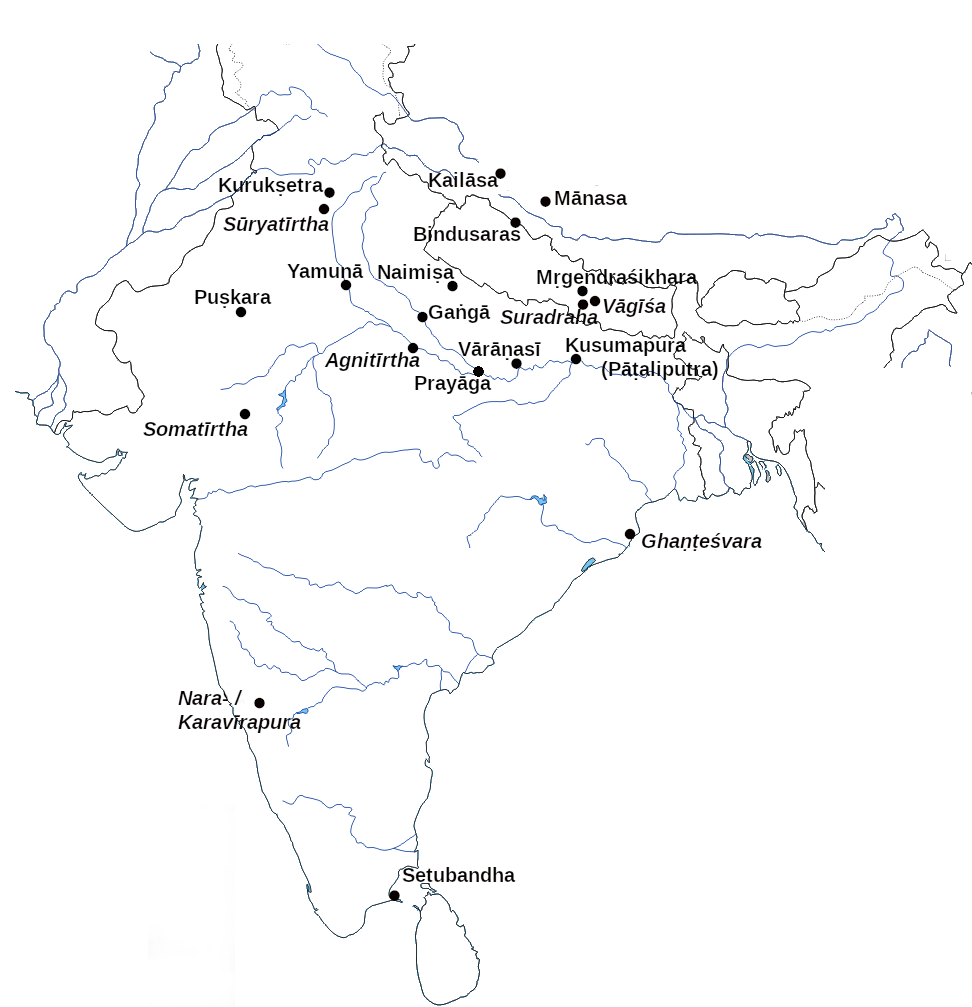
\includegraphics[scale=.5]{simplemap.png}
\caption[Geography of the \VSS]{A possible reconstruction of the  geography of the \VSS. Toponyms in italics are uncertain. Map constructed using a simple hydrographic map made by Daniel Dalet (d-maps.com).\label{fig:map01}}
\end{figure}

\thispagestyle{empty}
\begin{figure}[!]
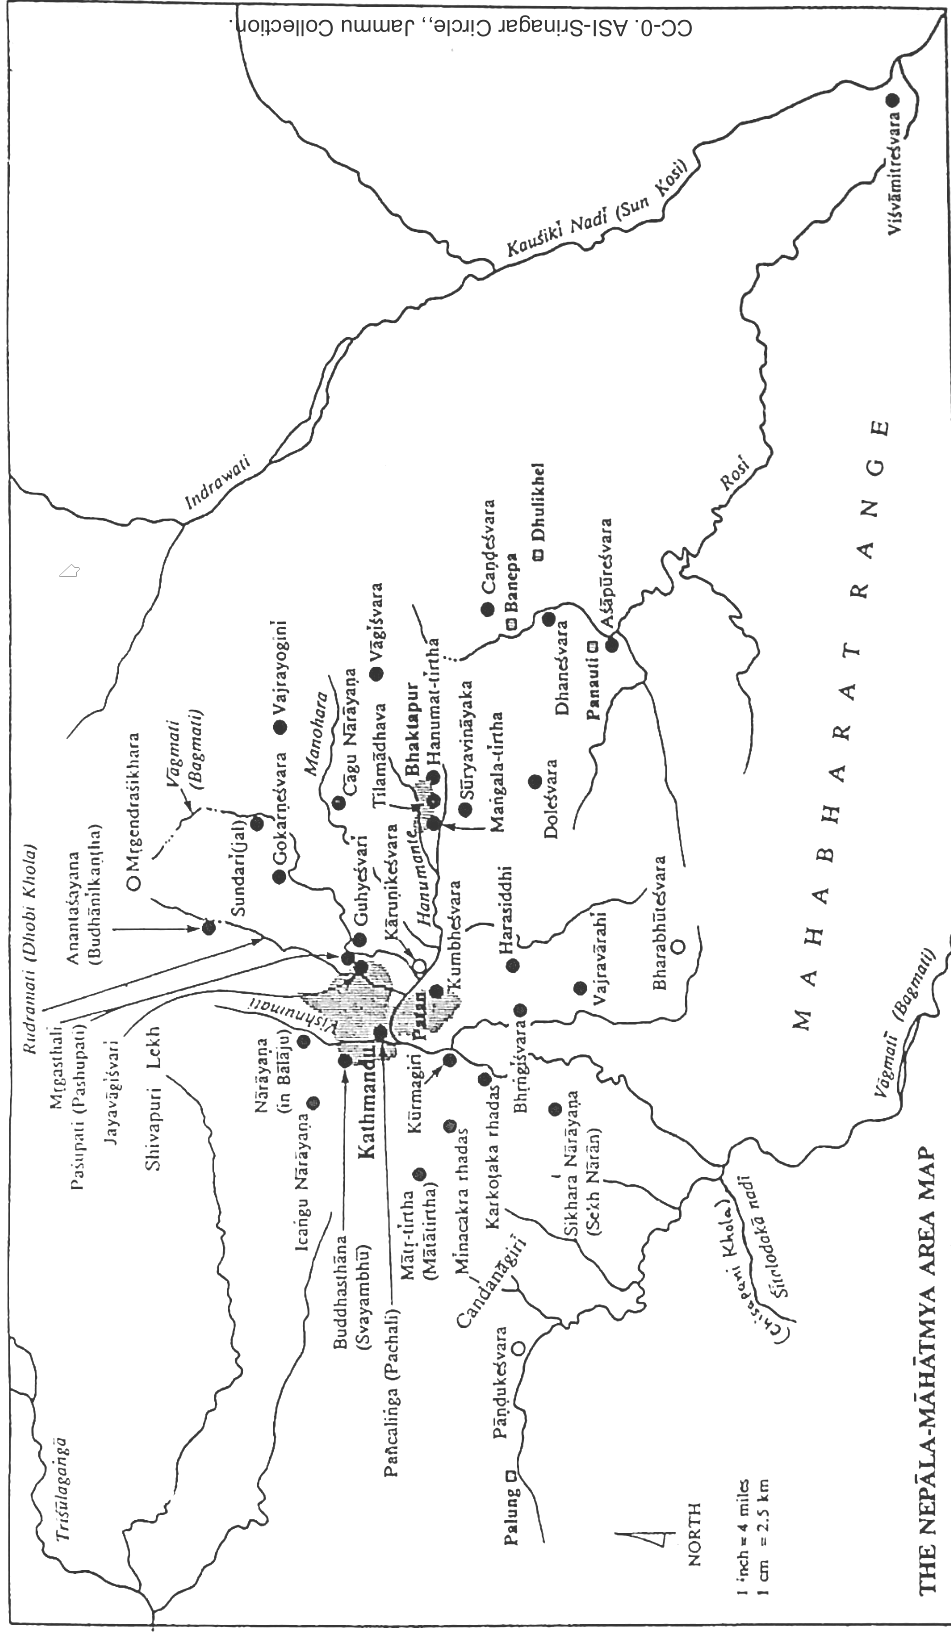
\includegraphics[scale=.43]{map_in_jayaraj.png}
\caption[Map in \mycite{AcharyaNepalaMahatmya}]{Map in \mycite{AcharyaNepalaMahatmya}
\label{fig:map02}}
\end{figure}


The location with which the ascetic Anarthayajña
is connected strongly suggests the Kathmandu 
valley as the geographical focus of the \VSS\
because he is a key figure and 
main interlocutor in the \VSS.%
	\footnote{On Anarthayajña's central role in the \VSS,
			see more in \mycite{KissVolume2021}.}

Turning to names of individuals mentioned in the \VSS,
those that might betray anything about the place or
time of composition of the text include King Siṃhajaṭa
and queen Kekayī, rulers of Nara- or Karavīrapura
in the narrative of chapter twelve. Unfortunately,
so far I have not been able to link these names to
any historical or legendary persons. The name of the
hero of the same chapter, Vipula, may be familiar 
from \MBH\ 13.40.16--13.43.16.: 

\begin{quote}
Devaśarman asks his disciple,
Vipula, to protect his wife, Ruci, primarily from Indra's
amorous advances, while he is away from home.
Vipula decides that the only way he can protect Ruci
is from within, i.e., by entering her body by yogic powers.
Vipula succeeds in protecting Ruci's reputation and 
departs to practise extreme austerities. Later he 
encounters several people (in fact,
as we learn later, Day and Night,
and the six seasons) who mention `Vipula's path to
the other world' (\skt{vipulasya pare loke yā gatis}, 
\MBH\ 13.42.27cd) as something horrible. He 
wonders what sins he may have committed that
could yield such unfortunate consequences. He
realizes that by not telling Devaśarman that he
actually entered Ruci's body, he lied and thus
may have commited a horrible sin. When Devaśarman learns
about this, he praises Vipula for his services instead, 
and all three, Devaśarman, his wife, and Vipula,
go to heaven.%
		\footnote{See a summary of Vipula's story in the 
			\MBH\ also in 
			\mycitep{SukthankarCriticalStudies}{317--318}.}
%(\MBH\ 13.43.16)
\end{quote}

\noindent
Thus, ironically, while the Vipula of the \MBH\ is famous
for protecting somebody else's wife,  
a rather different Vipula
in \VSS\ chapter twelve is somebody who donates
his wife to a Brahmin as soon as the latter expresses
his interest in her. It is more than possible that
the two characters have no connection at all.

Other characters in \VSS\ chapter twelve---Kapila, 
Vipula's father;
Bhīmabala, a traveller; Puṇḍaka, the foreman; 
and Caṇḍa and Vicaṇḍa, two royal envoys---seem 
to be of little use for us to ascertain the time and place of composition or redaction of the \VSS. 

As mentioned above, any discernible influence
of a local, vernacular language on the style or grammar of
a Sanskrit work could obviously be useful to 
locate the text in question geographically. 
The language of the \VSS\
displays numerous oddities that could be
explained by the interference of some other 
language, most likely early classical Newar.
On this, see a separate section below on 
pp.~\pageref{newar}\thinspace ff.

\medskip
As for the dating of the \VSS,
the \textit{terminus ante quem} for its
composition\thinspace /\thinspace redaction
the obvious date is the earliest MSS that transmits it.
The earliest dated MS that contains the \VSS\ is \msKoa. 
It is dated to Nepal Saṃvat 156, i.e., 1035-36 \CE.% 
	\footnote{See \mycitep{SastriCatalogue5}{721} and
		\mycitep{UmaSivaPlay}{591}. The date
	 	is clearly visible as `\skt{samvat} 156' 
	 	in the last line of the penultimate folio side 
	 	of \msKoa/8.}
In a multiple-text MS%
	\footnote{See more detail on this MS, which is
						now to be found in Munich, in	
					    \mycite{HarimotoMunichMS}.}
that is potentially earlier than \msKoa,
the \VSS\ is written in a hand that seems later than
that used for some of the other texts within the MS.%
		\footnote{\mycitep{HarimotoMunichMS}{597--598}:
		`This Śivadharma ms consists 
		of two major parts, easily distinguishable by different 		
		hands: one that appears to be produced in
		9th-c.\ Nepal [\dots], and another seemingly from 
		a century or so later [\dots] 
		The next set of folios making up this Śivadharma ms 	
		consists of three titles: the 
		\textit{Uttaromāmaheśvarasaṃvāda}* (24 folios), 
		the \textit{Vṛṣasārasaṃgraha} (50 folios), and the
		\textit{Dharmaputrikā} (11 folios). We do
		not know the original order of these three works 
		because each section starts with folio 1. Moreover, even 
		though these three titles appear to be written by the same 
		hand (probably somewhat later than the first part), there 
		is no certainty that these folios were produced to 	
		complement the first part.'}
The final colophon of the \VSS\ (and the \DHARMP) in
this MS  (\fol50r) is followed by the date
[Nepāla] `\skt{samvat} 192,' i.e., 1071-1072 \CE.

The above mentioned two MSS make it 
impossible to date the \VSS\ later than to the first
half of the 11th century \CE, and and parts of the text
could be considerably older that that period.
Archaic features that may indicate 
that the \VSS\ or parts of it were
composed much earlier than the early 11th century
include the following. Chapter ten, 
while it teaches the yogic tubes
\ie{nāḍī} Suṣumnā and Iḍā, is silent on Piṅgalā, 
which is a situation similar to that in 
the 6-7-century \Nisvnaya%
	\footnote{\mycitep{NisvasaGoodall}{33--35}.}  
(see details at the analysis of chapter 10 on 
pp.~\pageref{no_pingala} and in the notes to 
the translation).  Similarly, 11.23a 
(\skt{nivṛttyādi caturvedaś}) mentions four 
Śaiva \skt{kalā}s, instead of the expected and 
somewhat later, and in character tantric, five, namely
\skt{nivṛtti}, \skt{pratiṣṭhā}, \skt{vidyā}, 
\skt{śānti}, and \skt{śāntyatīta}. In the same chapter,
the order in which the \skt{āśrama}s are taught
(\skt{gṛhastha, brahmacārin, vānaprastha, parivrājaka}) 
is reminiscent of \Apastambadharmasutra\ 2.9.21.1,
and is relatively rare,
as opposed to the traditional order (\skt{brahmacārin,
gṛhastha, vānaprastha, parivrājaka}) found, e.g., in
\MANU. (See \mycitep{KissVolume2021}{195--196}.)
%cf. \mycitep{SaivaUtopia}{23}, Chapter 11, Śaiva
Another feature that might point towards a date
considerably earlier than the 11th century is the 
system of \skt{tattva}s in chapter 20:
the \skt{mahābhūta}s of classical Sāṅkhya are called 
\skt{dhātu}s here, the \skt{tanmātra}s of
classical Sāṅkhya are called \skt{guṇa}s,%
		\footnote{In contrast with, e.g.\ \SDHU\ 10.40--46 and
					\UUMS\ chapter 5, \DHARMP\ 1.42--43, or the \SIVAUP.}
the \skt{buddhi} of classical Sāṅkhya
is called \skt{mati}, and the highest \skt{tattva} 
is singular unlike the multiple \skt{puruṣa}s of classical 
Sāṅkhya. These may well be archaisms 
included in the \VSS\ consciously, but they could also
indicate that the time of composition of the \VSS\
is much closer to pre-classical Sāṅkhya than what the MS
evidence suggests.%
	\footnote{There are also numerous borrowings in \VSS\ 20
					from the Śāntiparvan of the \MBH. See more details
					at the analysis of \VSS\ chapter 20 in volume two.}

All in all, in light of all the above,
it is difficult to be more precise on the dating
of the \VSS\ than saying that its production must have
happened before the end of the 10th century---or beginning 
of the 11th century \CE\ if our oldest dated MS that trasmits
the \VSS\ is close in time to the actual composition or
redaction of the text. This could also mean a date considerably
earlier than the 10th century, and therefore a tentative dating
for the \VSS\ would be the 7th to 10th centuries \CE.
%    varṇas and the Liṅgapurāṇa
%    check lists of deities such as Vasus
%  bull, Nandi

\section{Authors, redactors and target audience}


\section{Why was the \VSS\ included in the Śivadharma corpus?}

One of the objectives of the article 
\mycite{KissVolume2021} was
to find clues about the r\^ole of the \VSS\ in the Śivadharma corpus.
The conclusion  therein (pp.~200--201), focusing on the fusion of 
Vaiṣṇava and Śaiva material in the \VSS, and on the reinterpretations of 
the \skt{āśrama} system in its eleventh chapter, includes the following:

\begin{quote}
The \Vss's role in the Śivadharma corpus is then twofold: 
it provides a text that is suitable for Vaiṣṇavas and Śaivas,
presenting its teachings on different levels of an esoteric scale, 
the Śaiva teachings being closest to the core, and always
providing an internalised, secret version of topics 
discussed in the other layers; and it also reinvents the traditional 
\skt{āśrama} system in a Śaiva way,
but in such a manner that would be acceptable for other religious groups. 
This may be an attempt to further develop an idea that appears in both 
the \SDhS\ and the \SDhU.
\end{quote}

\noindent
Indeed, one of the most striking feature of the \VSS\
is its structure in which Vaiṣṇava material surrounds
Śaiva teachings (see pp.~\pageref{structure}\thinspace ff. above). 
Even the title is not unambiguously Śaiva, as
we have seen (see pp.~\pageref{title} above).
Can we still say that this text is Śaiva? Does it
aim at a sort of balance of Vaiṣṇava and Śaiva
teachings? Does this duality reflect the 
religio\-political reality of the era?

MORE...

\section{Pāśupatas in the \VSS}

\section{Tantric influence?}
niśvāsa as sadāśiva in ch.~16; Niśvāsa uttarasūtra 5.50-51; see also Kafle Niśvāsamukha p.11ff; ibid. p.12: ``The term niśvāsa means sighing. Thus, an alternative meaning of the Niśvāsatattvasaṃhitā could also be a ``sighing tantra.'' To be more precise, a tantra that originated from the sighing of Śiva. This is to say, the speech of Śiva.''

\section{Buddhism in the \VSS}


\subsection{Misc}

  susūkṣma: Śivadharmottara 10.45cd--46: rudraḥ ṣaḍviṃśakaḥ proktaḥ
  śivaś ca paratas tataḥ \textbar{}\textbar{} 45 \textbar{}\textbar{}
  saptaviṃśatimaḥ śāntaḥ susūkṣmaḥ parameśvaraḥ \textbar{}
  svargāpavargayor dātā taṃ vijñāya vimucyate \textbar{}\textbar{} 
  46
  







\section{Language}\label{language}

\subsection{Newar influence?}
\label{newar}

The language of the VSS goes beyond the idiosyncrasies of epic Sanskrit.
It exhibits strong similarities to Śaiva Aiśa Sanskrit,% 
		\footnote{On Aiśa, see, e.g., \mycitep{GoodallKirana}{lxv\thinspace ff.}, 
								  \mycitep{TorzsokSYMthesis}{xxvi\thinspace ff.},
						          \mycitep{KissBraYa}{77--87}, 
						          \mycite{GerstmayrAisa}, 
						          \mycitep{HatleyBraYaVol1}{28ff.}} 
and it applies particular metrical licences and 
uses a special vocabulary, morphology and syntax.
The analysis of this language, ideally, would help us
confirm the identity of the author(s) or redactor(s) of the text, 
and our views on its place of composition. In fact, 
to feed a working hypothesis, I will mention parallelisms
between the language of the \VSS\ and early classical 
Newar---since the \VSS\ was most probably produced in the 
Kathmandu valley%
		\footnote{See pp.~\pageref{provenance}\thinspace ff.}%
---whenever possible. 
Of course, the assumable date
of the composition of the \VSS, which is without much doubt
early 11th century or before, does not allow much direct 
comparison with contemporary Newar language texts.%
	\footnote{The earliest dated Newar document is 
			the Ukū Bāhāḥ landgrand palmleaf manuscript from
			1114 \CE. See, e.g., \mycite{MallaUku}.}
Therefore I have to project a much later Newar grammar
onto an earlier and less well-known 
state of the language, which is not without risks.

In the following, I will only give a brief overview of the most
important phenomena. For details, see the observations 
on the constitution of the Sanskrit text in the footnotes 
to the translation, as well as the Index.


\subsection{Number and gender}\label{number}
One of the most evident deviation from Pāṇinian grammar in 
the text of the \VSS\ is a general disregard of grammatical concord 
as to number and gender.%
	\footnote{Compare Kölver's introductory remarks in
				   his investigation of `Newarized Sanskrit' (\mycitep{KolverErgative}{202})
					in the \SvayP\ thus (ibid. 192):
					
					\noindent
	          	`Number is often ignored
	          	
					[\skt{catvāro 'pi maṇḍalañ ca} 429,19 (cf.\thinspace 429, 21), 
					\skt{narāḥ pañcagatiñ ca na labhec ca} 428,12],
					
					\noindent
					as is gender
					
			[\skt{tvam ekam āgataṃ na hi} 464, 10 `only you have not come’; 
			\skt{°nāgakanyā \dots\ vṛṣṭipūrṇaṃ kṛtam} 470, 8 
					`the Nāga girl made (it) full of rain'],
				
				\noindent
				and case
				
				[\skt{manuṣyāḥ \dots\ tasmai \dots\ pūjitam} 426, 2 etc. 
				`men worshipped him; he was worshipped by people'; 
				\skt{bhavatām apy arthāya karomy upāyakam mayā} 452, 5 
				`I am making an expedient for your sake'].'}
See, e.g., a plural verb
(metri causa?) with a singular subject in \VSS\ 1.25ab:

\begin{quote}
\skt{rātryāgame pralīyante jagat sarvaṃ carācaram} 

When [Brahmā's] night falls, the whole moving and unmoving universe dissolve[s].
\end{quote}

\noindent
See a neuter plural participle picking up a 
neuter singular and a feminine singular noun in 1.61ab:

\begin{quote}
\skt{pramāṇaṃ nāma saṃkhyā ca kīrtitāni samāsataḥ}

The numbers [pertaining to] the measurements have been taught in brief.
\end{quote}

\noindent
This confusion, or often metrically forced disregard of standard Sanskrit
grammar, when dealing with number and gender, becomes almost
predictable when the noun phrase involves numerals.%
    \footnote{I am thankful to Judit Törzsök, who first pointed out to me
    the regular nature of the phenomenon itself as seen in the \VSS, and who 
    later drew my attention to the similar Newar grammatical rule
    (personal communication, Nov 29, 2023), which 
    led me to an investigation of a possible link between the Sanskrit of the \VSS\
    and classical Newar.}
See, e.g., verse 1.2cd:


\begin{quote}
\skt{parva cāsya śataṃ pūrṇaṃ śrutvā bhāratasaṃhitām}

\dots\ having listened to the \titleface{Mahābhārata}, 
to all its hundred section[s] \ie{parvan} \dots
\end{quote}

\noindent
Here one would expect either a plural genitive \ie{parvāṇāṃ śataṃ},
a compound \ie{śataparvāṇi}, or a plural accusative \ie{parvāṇi śataṃ}.
Similarly, \skt{gatiś ca pañca vijñeyāḥ} in 3.5a stands for
\skt{gatayaś ca pañca vijñeyāḥ} (`and the paths are to be known as five'), 
partly metri causa; and an interrogative quantifier (\skt{kati}, `how many?') can
trigger the same: \skt{gatis tasya kati smṛtāḥ} (3.1d; `how many are its path[s]?').
It is not without interest that classical Newar rarely applies
any plural marker in noun phrases with numerals.\label{singularwithnumerals}% 
	\footnote{See, e.g., \mycitep{JorgensenGrammar}{18}:
			`The plural ending is wanting where plurality is expressed 
			in other ways; thus always after numerals, and
			mostly after nouns denoting ``many, all'' '.
			 Incidentally, singular after numerals is also the norm in Modern Nepali,
									 and in other, even more distant languages
									 such as Hungarian.} 
Moreover in Newar, `nouns denoting inanimate objects 
are indifferent as to number.'%
	\footnote{\mycitep{JorgensenGrammar}{5 and 17}.}
A further clear example is verse 3.6cd:

\begin{quote}
\skt{tasya patnī mahābhāgā trayodaśa sumadhyamāḥ}

       He has thirteen beautiful wives with nice waists.
\end{quote}

\noindent
Here, with no variants in any of the MSS consulted, only the very end 
of the noun phrase \ie{sumadhyamāḥ} has the required 
plural ending. This again is what we often see in Newar.%
		\footnote{`Any case [\dots] and/or plural markers [\dots], as well as 
		postpositions [\dots], are added to the last constituent of the 
		N[oun ]P[hrase].' (\mycitep{OtterCourse}{11--12}.)
		E.g.: in the Newar phrase \skt{thwo khuṃ-na khaṅ-ā rājā-pani}
		(`these kings seen by the thief'), the only indication that
		multiple kings are involved is the plural marker \skt{-pani}
		at the end (ibid.).}
A good example of total number-blindness is 5.17cd: 

\begin{quote}
\skt{kīrtitāni viśeṣeṇa śaucācāram aśeṣataḥ}

\dots\ the practice of purity is definitely expounded in great detail.
\end{quote}

\noindent
Note that there would have been little problem in composing the same
line in standard Sanskrit, e.g., beginning with \skt{kīrtitaṃ ca\dots}
Instead, this line gives away something about the author's indifference
towards grammatical concord.%
		\footnote{Compare Kölver's remark on the phrase \skt{āgataḥ sarve nāgāḥ}
		in \SvayP\ (on p.~459 in \mycite{SastriSvayambhuP}):
		`this is a remarkable lack of sensitivity as to the category of number'
		(\mycitep{KolverErgative}{195}).}
Also, the participle \skt{kīrtitāni} might
function here as a finite verb in the plural: `they teach [the practice of purity].'
In this case there is some sense of number but coupled with a totally 
blurred boundary between finite verbs and participles.


In general, gender confusion is not unusual in epic Sanskrit and in Aiśa.%
		\footnote{See, e.g., \mycitep{OberliesEpicSkt}{XXXVIII--XL}, and
									\mycitep{KissBraYa}{85 and the Index therein}.}
It is its extent in the \VSS\ that suggests a very strong external influence,
supposedly of classical Newar.									





\subsection{Case and syntax}

An extreme example of a total lack of awarness of Sanskrit syntax is
\VSS~17.20:

\begin{quote}
\skt{bhūmipradātā dvija hīnadīnaḥ}\\
\skt{\phantom{aaa}samṛddhasasyo jalasaṃnikṛṣṭaḥ} |\\
\skt{sa yāti lokam amarādhipasya}\\
\skt{\phantom{aaa}vimānayānena manohareṇa} ||

        He who donates to a poor and distressed Brahmin land 
        that yields plenty of corn and is in the vicinity of water
        will go to the world of the king of the immortal ones [i.e.\ of Indra]
		 on a fascinating \ae rial vehicle.
\end{quote}            
            
\noindent            
The translation of this verse, surprising as it may seem, is, based on the
context, rather secure. \skt{Pāda}s ab probably stand for a sentence that would
be the following in slightly more standard Sanskrit:
\skt{yo dvijāya hīnadīnāya sasyasamṛddha-jalasaṃnikṛṣṭa-bhūmi-pradātā}.
This is expressed by a phrase in which a word that should be 
in the dative or genitive \ie{dvija} is in the vocative, and  
everything else is in the nominative: endings seem but
decorations. This is difficult to explain by classical Newar influence since Newar
does have a dative case marker, with animate nouns added to the genitive
marker. Similarly difficult is to explain why then \skt{pāda}s cd
are written in perfect standard Sanskrit.%
		\footnote{See a similarly puzzling situation in the \BraYa, 
						which is briefly described in \mycitep{KissBraYa}{74} as follows:
		`One of the most intriguing questions concerning the Bra[hma]Yā[mala] 
		is not why its language deviates from Pāṇini so often 
		but rather why sometimes it falls back to perfectly standard 
		Pāṇinian language for fairly long passages.'}

There are dozens, or hundreds, of syntactical oddities in the \VSS,
even if not all this baffling.%
		\footnote{Most of them are addressed in the footnotes 
									to the translation.}
Somewhat similarly to what Kölver describes in 
his analysis of the language of the \SvayP, a Nepalese composition (\mycite{KolverErgative}),
there often (but not always!) seems to be a lack of understanding of the
passive, together with the application of the ergative, one of the
basic syntactical tools of classical Newar. To demonstrate this, a good 
example is 12.113cd:

\begin{quote}
\skt{indreṇāsmi phalaṃ dattaṃ sa phalaṃ datta me bhavān} 

It was Indra who gave me the fruit and I gave that fruit to you.
\end{quote}

\noindent
Again, this is the translation that seems to fit the context. 
Here the skeleton of \skt{pāda} c is a well-constructed passive:
\skt{indreṇa phalaṃ dattaṃ}, but then, instead of adding a dative or 
genitive (e.g., \skt{indeṇa me phalaṃ dattaṃ}), the author chooses 
a finite verb (\skt{asmi}). In \skt{pāda} d, after seemingly 
treating \skt{phalaṃ} as a masculine noun, and leaving
\skt{datta} in stem form metri causa, and using \skt{me} for \skt{mayā},%
		\footnote{This often happens in epic Sanskrit, see 
			\mycitep{OberliesEpicSkt}{4.1.3, pp.~102--103}.}
this time ends the phrase with a noun in the nominative \ie{bhavān} instead of
the dative or genitive. Why not try to write \skt{dattaṃ tad eva te mayā},%
		\footnote{Although this solution carries the metric fault of 
								being iambic.}
or \skt{dattaṃ tava tad eva ca}?
Constructions with \skt{datta}/\skt{kathita} plus an expected dative 
are especially prone to confusion. See, e.g., \VSS\ 1.62cd--63ab and 
10.2d:

\begin{quote}
\skt{brahmaṇā kathitaṃ pūrṇaṃ mātariśvā yathātatham}\\
\skt{vāyunā pāda saṃkṣipya prāptaṃ cośanasaṃ purā}

        [The Purāṇas] were taught by Brahmā to 
        Mātariśvan [= Vāyu] in their entirety, in their true form.
        Vāyu abridged the verses and then gave [them] to Uśanas.
        
\skt{bravīmi vaḥ purāvṛttaṃ nandinā kathito 'smy aham}

        I shall teach you an ancient legend that Nandi told me.
\end{quote}

\noindent
Again, there is some struggle first with an expected dative here:
it ends up in the nominative \ie{mātariśvā}. Then an expected 
agent in the instrumental, or rather another dative, 
becomes an accusative \ie{cośanasaṃ}. Thirdly,
\skt{kathito 'smi} stands for \skt{kathitaṃ mama} or
\skt{kathitaṃ mahyam}. 

Somewhat similar are constructions with a 
past participle plus \skt{asmi}
in place of an active finite verb. See, e.g.,
13.68cd, 14.56ab and 15.15cd:

\begin{quote}
\skt{eṣa garbhasamutpattiḥ kathito 'smi varānane}

            This is how I have told you the formation of 
            the embryo, O Varānanā.
            
\skt{āgneyadhātuṃ somaṃ ca kathito 'smi varānane}

			I have taught, O Varānanā, the Fiery constituents 
			and the Soma-ones.
			
\skt{kathito 'smi samāsena kim anyac chrotum icchasi}

		Thus have I briefly described [to you, O Mahādevī, the soul.] 
		What else would you like to hear?
\end{quote}

\noindent
These are also similar to what \citeauthor{JorgensenVicitra}
analyses in a Sanskrit passage in the Newar
\titleface{Vicitra\-karṇikāvadā\-noddhṛta}, namely that
the phrase \skt{na jñāto 'ham} must in that context 
mean `I did not know.'%
		\footnote{\mycitep{JorgensenVicitra}{77 and 328}.
						Compare \skt{tat phalaṃ sa niveditaḥ} (`he gave that fruit') in \VSS\ 12:67d.}

%Vicitrakar :
%ibid and 66 \skt{aṣṭhan/au divasam āgata} should mean `Come on the eighth day'.;
%buddhamārgaṃ abhijñātaṃ: `on the well-known path of the Buddhas'
%80 and 328-329 samagraṃ, stem forms etc.!?

Sometimes the agent an active construction with a transitive verb
simply imitates an ergative structure: \skt{viṣṇunā\dots\ papraccha} (1.8),
\skt{sa}[!] \skt{hovāca pathīkena} (12.60a).%
		\footnote{This happens also in Aiśa. See, e.g., \SiddhYogMata\ 18.23: 
		\skt{pūjayet \dots\ mantriṇā} (\mycitep{TorzsokSYMthesis}{42}).}

Another typical syntactical construction in the \VSS\ is a verb
meaning `to tell, teach' plus a noun in the genitive, e.g. 4.69ab:

\begin{quote}
\skt{caturmaunasya vakṣyāmi śṛṇuṣvāvahito bhava}

        I shall tell you about the four cases of observing silence. 
        Listen, be attentive.
\end{quote}

\noindent
One could say that \skt{pāda} a is simply elliptical and that
a verb like \skt{lakṣaṇaṃ} or \skt{svabhāvaṃ} 
(`the caracteristics/essence [of X]') is missing. 1.37ab is similar:

\begin{quote}
\skt{brahmāṇḍānāṃ prasaṃkhyātuṃ mayā śakyaṃ kathaṃ dvija}

How could I enumerate [all the details of] the Brahmāṇḍa[s], O twice-born?
\end{quote}

\noindent
This phenomenon is difficult to explain by any Newar influence since
classical Newar would usually also require an 
extra word (such as \skt{khaṃ} `thing, topic, word, story') in such a sentence.
It might belong to a class of phenomena in Buddhist Hybrid Sanskrit 
that Edgerton labels as `Genitive with miscellaneous verbs.'%
		\footnote{\mycitep{EdgertonHybrid}{vol.~1, \S 7.65, p.~47}.}

These kinds of deviations from standard Sanskrit make it
necessary that the translation be somewhat intuitive,
driven by the context, rather than by an analysis of syntax.

%as if not proofread



yajec cakre ca vidhivad yoginīsiddhim icchatā 21.12cd


\subsection{Cardinal and ordinal numbers}

Although the \VSS\ does use simple ordinal numbers such 
as \skt{prathama}, \skt{dvitīya}, and \skt{tṛtīya}, with higher 
numbers there seems to be a non-distinction between cardinal
and ordinal numbers, and cardinals are used as ordinals.
See, e.g., 20.8ab and 11ab:

\begin{quote}
\skt{caturviṃśati yat{ }tattvaṃ prakṛtiṃ viddhi niścayam}\\
\skt{dvāviṃśati ahaṃkāras{ }tattvam{ }uktaṃ manīṣibhiḥ}

Know the twenty-fourth Tattva certainly as Prakṛti.
The twenty-second Tattva is Ahaṃkāra according to the wise.
\end{quote}

\noindent
This phenomenon is known to a certain degree
from epic Sanskrit,%
	\footnote{See \mycitep{OberliesEpicSkt}{\S 5.2.2, pp.~127--128}.}
and is even more characteristic of classical Newar.%
		\footnote{See \mycitep{JorgensenGrammar}{42} and
									 \mycitep{OtterCourse}{57}.}





\subsection{Stem form nouns}\label{stemform}

Stem form nouns, or \skt{prātipadika}s, are extremely common in the
language of the \VSS. They are not alien to the Aiśa Sanskrit
of Śaiva Tantras,%
		\footnote{See, e.g., \mycitep{KissBraYa}{75--77} and
								\mycitep{NisvasaGoodall}{126 and 441}.}
but the extent to which they prevail in the \VSS\ is striking and it
reminds one of the zero suffix of the nominative and accusative,
or rather of the `casus indefinitus' or `absolutive case' of classical Newar.%
		\footnote{\mycitep{JorgensenGrammar}{18 and 21},
		 and \mycitep{OtterCourse}{16}.} 
Often stem forms are required to restore the metre, 
and they would thus be difficult to emend,
and often they blend in sandhi with the following word. 
See some clear examples below with the expected, 
but usually unmetrical, form in parentheses:

\begin{quote}
 1.63a: \skt{vāyunā pāda saṃkṣipya} (\skt{pādaṃ}) \\
1.63c: \skt{tenāpi pāda saṃkṣipya} (\skt{pādaṃ}) \\
2.25c: \skt{bhogam akṣaya tatraiva} (\skt{akṣayaṃ}) \\
2.26d: \skt{īśānānāṃ smṛtālayaḥ} (\skt{smṛta ālayaḥ}) \\
4.19f: \skt{prasahyasteya pañcamam} (°\skt{steyaṃ}) \\
4.72a: \skt{caturdhyānādhunā} (°\skt{dhyānam adhunā}) \\
4.77a: \skt{pramādasthāna pañcaiva} (°\skt{sthānaṃ} or °\skt{sthānāni})
 \\
6.5c: \skt{vedādhyayana kartavyaṃ} (\skt{vedādhyayanaṃ}) \\
6.14a: \skt{dvitīyaṃ tattva puruṣaṃ} (\skt{tattvaṃ}) \\
\end{quote}





\subsection{Vocabulary}




  Special vocabulary/language: karhacit, hṛdi as nominative 10.27cd,
  tirya, me as mayā, āhūtaplavana

  generate list from index

Modern Nepali: singular after numerals.

Kölver

No short-long


\subsection{Metre}\label{metre}
\label{muta}
As regards metrical licences, perhaps 
the most striking feature is the generous
use of the poetic licence sometimes labelled `muta cum liquida,'%
	\footnote{For a recent contribution on this phenomenon, see,
 	 \mycite{SenMutaCum} (discussing it as it appears in Latin).}
 	%and \mycitep{BaloghYati}??  2018, note 6 (discussing 
 	%Sanskrit metre), Balogh 2019, 39 and 115
namely that some consonant clusters that would 
normally turn the previous short \ie{laghu} syllable
long \ie{guru} may in some cases do not do so.%
		\footnote{On its appearance in Śaiva Tantras,
							see, e.g., \mycitep{GoodallParakhya}{lxxxi} and
							\mycitep{NisvasaGoodall}{441}.}
Syllables beginning with \skt{pr, br, hr, kr}, 
especially (or exclusively?) at the beginning of words, are well-known
candidates for this licence.%
			\footnote{See, e.g., \mycitep{ApteDict}{Appendix~A p.~1}.} 
In the \VSS, \skt{tr, vr, śr, pr}, and also 
\skt{śy, śv, sv, dv},%
	\footnote{See, e.g., the cadence of 5.15b: \skt{śukaśyenakān} for \ \shortsyllable\ 
								\shortsyllable - \shortsyllable -}
can also trigger this licence. 
All these syllables involve conjunct consonants with
a semivowel in second position.
% and possibly also rpa,CHECK! seem additional ones.

For context, it is perhaps not useless to briefly show
what a well-known author on prosody, 
Kedārabhaṭṭa (11th or 12th century),%
		\footnote{\mycitep{OllettGana}{333}.}
who is frequently quoted by Mallinātha, has to say on this
phenomenon in his
\skttitle{Vṛttaratnākara}{Vrttaratnakara} (here given together with Sulhaṇa's \skttitle{Sukavihṛdayanandinī}{Sukavihrdayanandini} commentary):%
		\footnote{\mycite{PatelVrttaratnakara}.}

\begin{quote}
\skt{padādāv iha varṇasya saṃyogaḥ kramasaṃjñikaḥ} | \\
\skt{puraḥsthitena tena syāl laghutā 'pi kvacid guroḥ} || 1.10 ||

In this [work], a combination of two or more consonants
\ie{saṃyoga} in a word-initial syllable \ie{pādādau varṇasya} is
called `sequence' \ie{krama}. [A syllable that counts as] long because one
such [consonant cluster] stands in front [of it, i.e.\ after it] can 
sometimes be treated as short.

{\footnotesize [Comm.:] 
\skt{vibhaktyantaṃ padaṃ tasya padasyādau vartamāno yo varṇas tasya
saṃyogaḥ} | 
\skt{sa iha śāstre kramasaṃjño jñeyaḥ} |
\skt{tena krameṇa purovartinā prākpadānte vartamānasya
prāptagurubhāvasyāpi laghutā syāt} | 
\skt{kvacil lakṣānurodhena} | 
\skt{nanu ka eṣaḥ kramo nāma saṃyoga ucyate} | 
\skt{pūrvācāryāṇāṃ piṅgalanāgaprabhṛtīnāṃ kālidāsādīnāṃ ca
kavīnāṃ samayaḥ parigṛhītaḥ} |
\skt{saṃyogaḥ kramasaṃyogaḥ}
|| 10 || 
\skt{tatra gra-saṃyogena yathā} | 
\skt{idam asyodā\-hara\-ṇam}~|

A `word' is [a unit of speach that] ends in an inflection. 
A `conjunction' is in a `syllable' which is
at the beginning of such a word. 
`In this' [i.e.] work it is to be known under the 
term `sequence' \ie{krama}. By that sequence which stands in front, 
[a syllable] at the end of the previous word, even if it acquired
heaviness [by position], may acquire lightness. `Sometimes' [means:]
according to the examples.
But then what is this combination of consonants called `sequence'?
The old teachers such as Piṅgalanāga and poets such as Kālidāsa
accepted [this] rule. The combination of consonants \ie{saṃyoga}
is [here] the sequence[-type] \ie{krama} [i.e. word-initial] 
combination of consonants \ie{saṃyoga}.
Among [the possibilities,] for example by conjunct consonant 
\skt{gr}.
Here is an example of that:}

\skt{taruṇaṃ sarṣapaśākaṃ navaudanaṃ picchalāni ca dadhīni} |\\
\skt{alpavyayena sundari grāmyajano miṣṭam aśnāti} || 1.11 ||

Tender mustard seed, fresh porridge, and slimy curds: men in the village eat
these kinds of savoury dishes, O pretty girl, because they do not have
much money.%
	\footnote{I.e.: `you are pretty, don't waste your time with poor village men.'}
\end{quote}

\noindent
The example verse given above (1.11) is in \skt{āryā}, and the
metric pattern of the second half-verse is, strictly speaking, the following:
 
- - | \shortsyllable\ - \shortsyllable\ | - \shortsyllable\ -!~| 
- \shortsyllable\ \shortsyllable\ | 
- - | \shortsyllable\ | -  - | - |

This is unmerical and it yields 28 mor\ae, instead 
of the expected 27. By treating the final syllable of \skt{sundari} short, 
in spite of the following \skt{grā}, the pattern conforms 
to the expected pattern: 

- - | \shortsyllable\ - \shortsyllable\ | 
- \shortsyllable\ \shortsyllable\ | - \shortsyllable\ \shortsyllable\ | - - | 
\shortsyllable\ | - - | - |

The commentator gives several more examples, involving the syllables
\skt{gra}, \skt{hra}, and \skt{bhra}, and confirms that the rule
applies only to word-initial consonant clusters: 

\begin{quote}
{\footnotesize\skt{padādāv iti kim | anyatra mā bhūt |}

Why `at the beginning of a word'? [Because] elsewhere it should not be.}
\end{quote}

\noindent
Here follow some examples from the \VSS. The syllables 
with the \skt{krama} conjunct consonant, before which the syllable 
is not turned into long, are encircled, and the metre is given in 
parentheses.

\begin{quote}	
1.1c: \skt{harīndra\Circled{br}ahmādibhir āsamagraṃ} (\skt{upajāti})\\
4.67c: \skt{prajñābodha\Circled{śr}utiṃ smṛtiṃ ca labhate mānaṃ ca nityaṃ labhed} (\skt{śārdūlavikrīḍita})\\
4.89a: \skt{iti yama\Circled{pr}avibhāgaḥ kīrtito 'yaṃ dvijendra} (\skt{mālinī})\\
5.5cd: \skt{parastrīpara\Circled{dr}avyeṣu śaucaṃ kāyikam ucyate} (\skt{pathyā})\\
5.9cd: \skt{vānaprasthasya \Circled{tr}iguṇaṃ yatīnāṃ tu caturguṇam}  (\skt{na-vipulā})\\
5.15ab: \skt{haṃsasārasacakrāhvakukkuṭān śuka\Circled{śy}enakān} (\skt{pathyā})\\
8.33a: \skt{tasmān mauna\Circled{vr}ataṃ sadaiva sudṛḍhaṃ kurvīta yo niścitaṃ} 
 (\skt{śārdūla\-vikrīḍita})\\
10.31b: \skt{īśānenābhijuṣṭaṃ hṛdi \Circled{hr}ada vimalaṃ nādaśītāmbupūrṇam} (\skt{srag\-dharā})\\
11.9ab: \skt{manaḥśuddhis tu \Circled{pr}athamaṃ dravyaśuddhir{ }ataḥ param} (\skt{na-vipulā})
\end{quote}

\noindent
These indeed follow the rule of having the special conjunct with the semi\-vowel
at the beginning of a word in the sense that the word can be a member
of a compound.%
		\footnote{There are some problematic verses that I ignore here. They are
						unlikely to change the overall picture.}
To understand how unique the \VSS's indulgence in the `muta cum liquida'
licence is, the epics and the Purāṇas should be examined from this 
perspective.						

Another metrical odditity, or rather metrical licence, that is applied
regularly in the \VSS, exclusively in non-\skt{anuṣṭubh} verses,
 is that a word-final short syllable can count 
as long. Here are some examples, with the short syllable now
turned into long encircled:

\begin{quote} 
3:42d: \skt{etatpuṇyapha\Circled{la}m ahiṃsakajanaḥ prāpnoti niḥsaṃśayaḥ} 
 (\skt{śā\-rdū\-la\-vikrīḍita})\\ 
 4.5a: \skt{na narmayu\Circled{kta}m anṛtaṃ hinasti} (\skt{upajāti})%
 		\footnote{Versions of this line in the \MBH\ and the \MATSP\
 								read °\skt{yuktaṃ vacanaṃ} (see the apparatus
 								at veres 4.5 in the edition).}\\
4.39c: \skt{aśeṣaya\Circled{jña}tapadānapuṇyaṃ}  (\skt{upajāti})\\
4.59c: \skt{vijñānadha\Circled{rma}kulakīrtināśa} (\skt{upajāti})\\
4.59d: \skt{bhavanti vi\Circled{pra} damayā vihīnāḥ} (\skt{upajāti})\\
5.20a: \skt{śaucāśaucavidhijña mānava ya\Circled{di} kālakṣaye niścayaḥ} (\skt{śā\-rdū\-la\-vikrī\-ḍita})\\
6.18b: \skt{jijñāsyantāṃ dvijen\Circled{dra} bhavadahanakaraḥ prārthanā\-kalpa\-vṛkṣaḥ} (\skt{sragdharā})\\
7.13b: \skt{saubhā\Circled{gya}m atulaṃ labheta sa naro rūpaṃ tathā śobhanam} (\skt{śā\-rdū\-la\-vikrīḍita})\\
8.44d: \skt{na bhavati punaja\Circled{nma} kalpakoṭyāyute 'pi} (\skt{mālinī})\\
11.42b: \skt{saṃsāroddhara\Circled{ṇa}m anityahara\Circled{ṇa}m ajñānanirmūlanam} (\skt{śā\-rdū\-la\-vikrīḍita})\\
11.42c: \skt{prajñāvṛddhika\Circled{ra}m amoghakaraṇaṃ kleśārṇavottāraṇaṃ} (\skt{śā\-rdū\-la\-vikrīḍita})\\
11.42d: \skt{janmavyādhiha\Circled{ra}m akarmadahanaṃ sevet sa dharmottamam} (\skt{śā\-rdū\-la\-vikrīḍita})\\
12.150c: \skt{nityaṃ rogādhivā\Circled{sa}m aniyatavapuṣaṃ trāhi māṃ kālapāśāt} (\skt{srag\-dharā})
\end{quote} 



  

%\CHECK  a more or less full collation is important: we cannot automatically reject `ungrammatical' or unmetrical forms because they may well be  the `original' one

\CHECK the more original a section the more extreme language? see ch11


\vfill
\pagebreak


\section{Contents and analysis of chapters 1--12}\label{contentsof1_12}

Here follow short descriptions of the topics found in chapters 1--12
of the \VSS---edited and translated in this volume---accompanied 
by brief discussions and analyses.%	
		\footnote{See a Sanskrit summary of the 
					contents of the \VSS,
				    based on Naraharinath's edition,
					in \mycitep{AnilkumarBook}{61--72}\verify. }
					
\subsection{Adhyāya 1}\label{contents_of_ch01}
After a \skt{maṅgala}-verse that addresses a 
deity whose identity is obscure (is it Śiva or the 
impersonal Brahman?; verse 1.1), we enter the first layer 
of the text, which comprises a dialogue between Janamejaya and 
Vaiśampāyana and could be labelled Dharmaśāstric.
Janamejaya wishes to hear the essence, the ultimate Dharmic teaching, 
of the \MBh. In response, Vaiśampāyana starts relating 
a dialogue during which Viṣṇu, diguised as a Brahmin, 
tests an ascetic called Anarthayajña, reknown for performing 
non-material sacrifice (\skt{anarthayajña}, 
the topic of \skt{adhyāya} eleven), and 
a devotee of Viṣṇu (which becomes clear in \skt{adhyāya} twenty-one). 
This is the beginning of the layer one could label Vaiṣṇava. 
The first topic they discuss is \skt{brahmavidyā} (1.9--10), and 
ambiguous definition of the impersonal Brahman and/or the syllable \skt{oṃ}. 
The next topic is \skt{kāla} (`death, time'), the origin of the body, karma (1.11--17), 
and the divisions of time (from \skt{truṭi, nimeṣa} up to \skt{kalpa}s, 1.18--30), 
which leads to a teaching on numbers, from one up to 
two hundred quadrillion (\skt{para}, 1.31--35).
Verses 1.36--39 introduce a list of the rulers of the eight 
regions of the Brahmāṇḍa (1.40--48). 
In addition, Viṣṇu features as the ruler of the centre of the Brahmāṇḍa (1.49),  
reconfirming the general Vaiṣṇava character of this layer. 
1.50--57 give the number of subordinates to each ruler mentioned above. 
1.58--61 teaches the measurements of the Brahmāṇḍa. 
Finally, verses 1.62--75 list the redactors and transmitters of the Purāṇas, 
from Brahmā to Vyāsa Dvaipāyana, Romaharṣa, and Romaharṣa's son Amitabuddhi.

 Keywords: Brahmā, Brahman
%
% 11:35:18 From somadeva vasudeva To Everyone : There is a very relevant forthcoming study by H. Kondo: “Fault Lines of Samkya History: Struggling with the Conflict between Satkarayvada and the Accumulation Theory” where he analyses exactly the differing accounts of the exact role of the tanmatras, using also Chinese sources. Hopefully our Journal will be able to publish it this year.
%11:40:18 From somadeva vasudeva To Everyone : Kenji can tell you more, but for dating also consider the Carakasamhita’s “samkhya section”.
%11:46:25 From Balogh Dániel To Everyone : Thanks for the talk. Must go. Have fun discussing.
%11:59:03 From somadeva vasudeva To Everyone : PS: can you maybe share the musicological section? Since musicological theory changes very quickly it might help with dating (if it is detailed enough).
%12:00:40 From Csaba Kiss To Everyone : Shareing the chapter in these formats:
%https://filedn.com/lFSw9FGgUBpyrpsGtImyUHh/vrsasarasamgraha/individual_chapters/vrsasara_ed_devnag20.pdf
%12:00:56 From Csaba Kiss To Everyone : https://filedn.com/lFSw9FGgUBpyrpsGtImyUHh/vrsasarasamgraha/individual_chapters/vss_chapter20.html
%12:02:18 From Yuko Yokochi To Everyone : Three grāmas are in the Nāṭyaśāstra.
%12:03:10 From somadeva vasudeva To Everyone : Check maybe also the B.rhadde”sii of Matas”nga
%12:03:16 From Sathyanarayana Sarma To Csaba Kiss(Privately) : Sorry Csaba, I had other reading, so I couldn’t join.
%12:04:55 From serenasaccone To Everyone : Thanks for the talk and lively discussion! Have to go. See you soon!
%12:11:38 From Csaba Kiss To Sathyanarayana Sarma(Privately) : https://filedn.com/lFSw9FGgUBpyrpsGtImyUHh/textprocess_javascript.html
%12:12:05 From Csaba Kiss To Sathyanarayana Sarma(Privately) : (Another approach at the above link.)

 
\subsection{Adhyāya 2}\label{contents_of_ch02}
Perhaps a later, tantric, insertion?

  2. śivāṇḍasaṃkhyā 

\subsection{Adhyāya 3}\label{contents_of_ch03}
  yamas-niyamas: see table in \mycitep{SaivaUtopia}{17}

\subsection{Adhyāya 4}\label{contents_of_ch04}
\subsection{Adhyāya 5}\label{contents_of_ch05}
\subsection{Adhyāya 6}\label{contents_of_ch06}
\subsection{Adhyāya 7}\label{contents_of_ch07}
\subsection{Adhyāya 8}\label{contents_of_ch08}
\subsection{Adhyāya 9}\label{contents_of_ch09}
\subsection{Adhyāya 10}\label{contents_of_ch10}
\label{no_pingala}

\subsection{Adhyāya 11}\label{contents_of_ch11}
\subsection{Adhyāya 12}\label{contents_of_ch12}

  3. ahiṃsāpraśaṃsā 
  4. yamavibhāga
  5. śaucācāravidhi
  6. yajñavidhi (also lokāḥ)
  7. dānapraśaṃsā 
  8. niyamapraśaṃsā (p. 603: types of svādhyāyana: śaiva, sāṃkhya, purāṇa,
                    smārta, bhārata)
  9. traiguṇyaviśeṣaṇīya
  10. kāyatīrthavivarṇana
  11. caturāśramadharmavidhāna 
  12. vipulopākhyāna  (narrative)
  13. garbhotpatti (on conception)
  14. praśnavyākaraṇa (why people are tall/short etc.)
  15. jīvanirṇaya 
  16. adhyātmanirṇaya (yoga) 
  17. dānadharma
  18. pūrvakarmavipāka
  19. dānayajñaviśeṣa
  20. pañcaviṃśatitattvanirṇaya
  21. kalpanirṇaya
  22. varṇagotrāśrama
  23. nidrotpatti
  24. śāstravarṇana


    everybody is donating to everybody,
  
    the final donor is Brahmā
  
    lot of testing going on in the frame story and also
  
    in chapter 12
  
    also the disguise thing is recurring: 12.37 and ch 1 and
  
    when Viṣṇu reveals his identity
    

\section{Topics in chapters 13--24}\label{contentsof12_24}

\vfill
\pagebreak
